\section{Circuitos Integrados com Amplificadores Operacionais}
\label{sec:circuitos_integrados}
Temos disponíveis no repositório 3 modelos de CI portador de amplificador operacional: \textbf{uA741, LM358 e LM324}. As peculiaridades de cada um serão descritas no fio abaixo, respectivamente:
\begin{enumerate}
    \item O CI uA741 possui apenas um amplificador operacional. Possui entradas de ajuste de \emph{offset}, para eliminar as variações de tensão entre as entradas inversora e não inversora do amplificador operacional. A alimentação é feita a partir de uma alimentação $V_{cc+}$ e $V_{cc-}$, onde ambos os valores devem ser iguais, com o sinal oposto. A disposição dos pinos do CI estão na figura \ref{fig:ua741}.
    \begin{figure}[H]
        \centering
        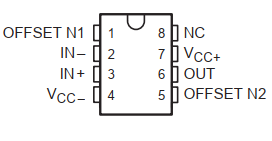
\includegraphics{imagens/ua741.png}
        \caption{Pinagem do CI uA741}
        \label{fig:ua741}
    \end{figure}
    
    \item O LM358 possui dois amplificadores operacionais, A e B. Eles não possuem ajuste de \emph{offset}. A alimentação é feita de dois modos: alimentando $V^+$ com 3V até 32V e GND aterrado, ou alimentando $V^+$ com +1.5V até +16V e GND com -1.5V até -16V, ambas as alimentações das entradas devem ser idênticas com sinais opostos. O arranjo dos pinos está disposto na figura \ref{fig:lm358}.
    \begin{figure}[H]
        \centering
        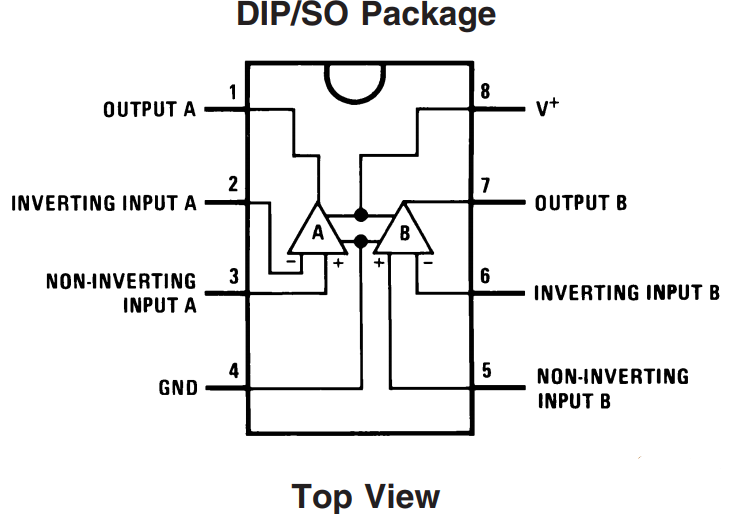
\includegraphics[width=.4\linewidth]{imagens/LM358.png}
        \caption{Pinagem do CI LM358}
        \label{fig:lm358}
    \end{figure}
    
    \item O terceiro CI, LM324, se dispõe de quatro amplificadores operacionais. Também não possui ajuste de \emph{offset}. A alimentação é feita da mesma forma que o CI LM 358. A pinagem utilizada é mostrada na figura \ref{fig:lm324}.
    \begin{figure}[H]
        \centering
        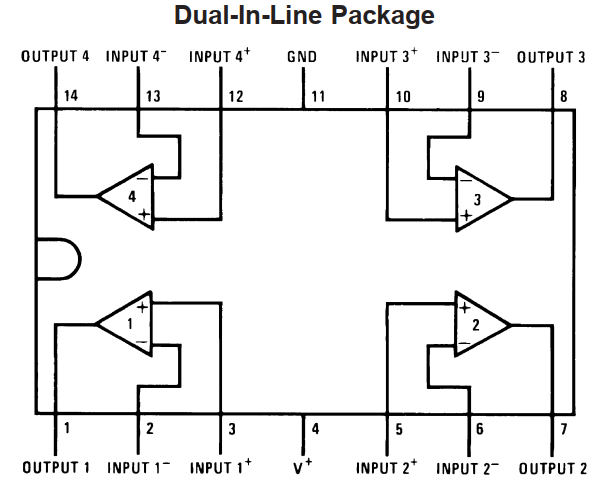
\includegraphics[width=.4\linewidth]{imagens/LM324.png}
        \caption{Pinagem do CI LM324}
        \label{fig:lm324}
    \end{figure}
\end{enumerate}
